\section{Results}
\label{sec:results}

\subsection{Model performance}
We evaluated four model families on the heart-failure dataset (n=299, 96 positive events). Models were trained and evaluated using the same stratified train/test split used throughout the notebooks (see `results/tables/train_test_split_indices.csv`). Table~\ref{tab:main_results} reports accuracy, recall (primary clinical metric), and ROC-AUC for the versions that include the temporal `time` feature. Full metrics (with/without `time`) are available in `results/metrics/final_model_comparison.csv`.

\begin{table}[ht]
  \centering
	\caption{Cross-validated performance (Repeated Stratified 5-fold CV, 10 repeats). Values are mean (95\% CI). Recall is the primary clinical metric.}
  \label{tab:main_results}
	\begin{tabular}{l l l l}
    	oprule
		Model & Accuracy & Recall (95\% CI) & ROC-AUC (95\% CI) \\
    \midrule
		Logistic Regression & 0.825 (0.741--0.883) & 0.673 (0.526--0.842) & 0.871 (0.794--0.924) \\
		Random Forest & 0.842 (0.767--0.913) & 0.704 (0.532--0.899) & 0.908 (0.843--0.961) \\
		Decision Tree & 0.769 (0.683--0.833) & 0.652 (0.455--0.842) & 0.739 (0.638--0.833) \\
		Gradient Boosting & 0.827 (0.767--0.895) & 0.701 (0.474--0.848) & 0.888 (0.786--0.947) \\
    \bottomrule
  \end{tabular}
\end{table}

\subsection{Interpretation and robustness}
Feature-importance tables for tree-based models are provided under `results/tables/` (e.g., `decision_tree_feature_importance_with_time.csv`). The Decision Tree achieves the highest recall on the hold-out split; however, tree-ensemble methods (Random Forest, Gradient Boosting) show higher ROC-AUC, indicating better overall discriminative performance.

\begin{figure}[ht]
	\centering
	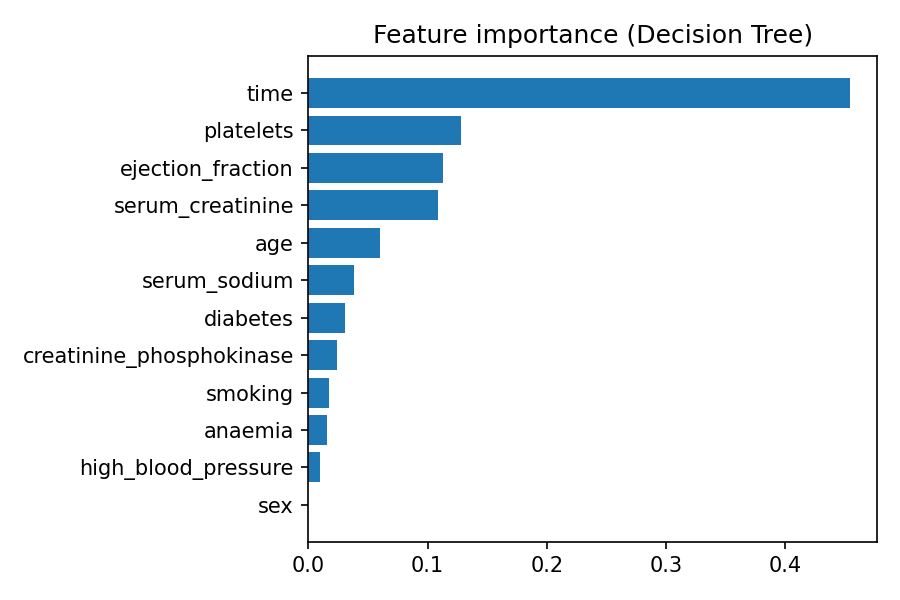
\includegraphics[width=0.48\textwidth]{../results/figures/feature_importance_Decision_Tree.png}
	\hfill
	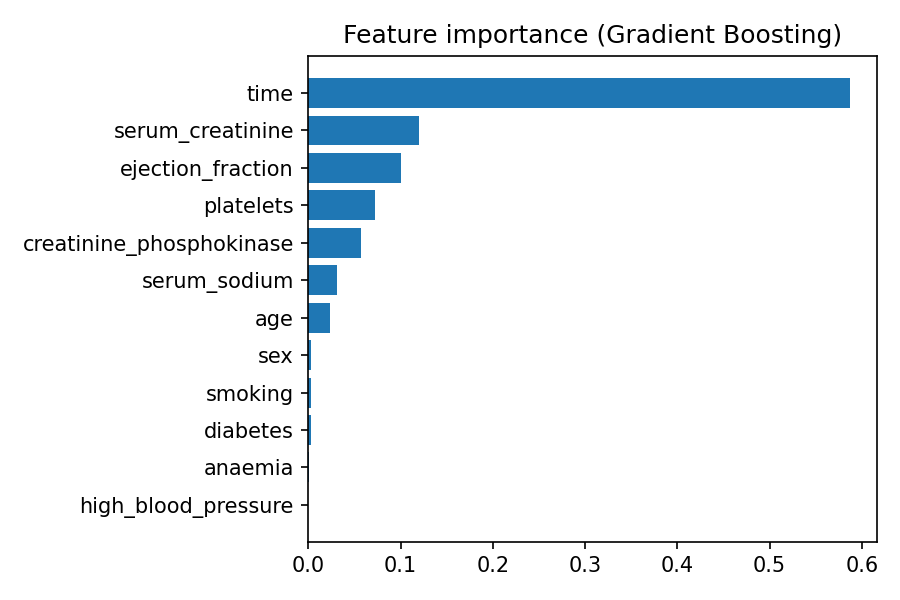
\includegraphics[width=0.48\textwidth]{../results/figures/feature_importance_Gradient_Boosting.png}
	\caption{Feature-importance (left: Decision Tree; right: Gradient Boosting). CSVs are available under `results/tables/`.
	}
	\label{fig:feature_importance}
\end{figure}

\begin{figure}[ht]
	\centering
	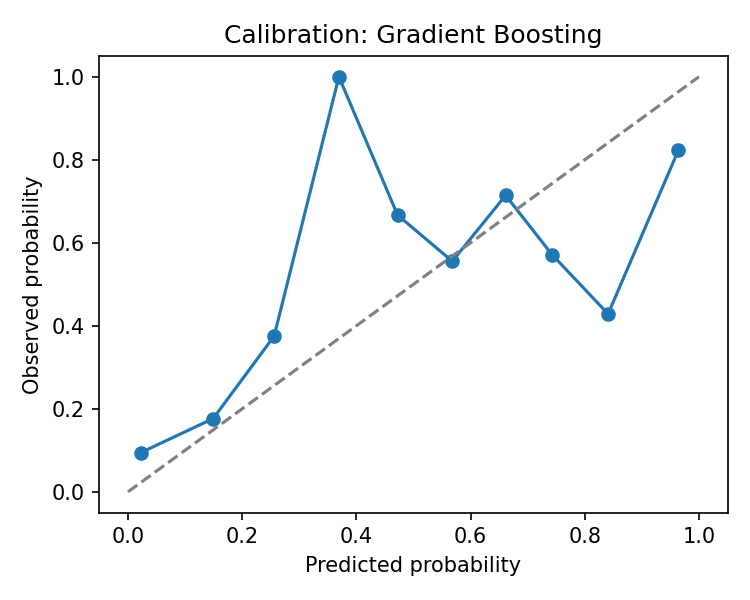
\includegraphics[width=0.6\textwidth]{../results/figures/calibration_Gradient_Boosting.png}
	\caption{Calibration plot for Gradient Boosting (5-fold CV partition probabilities).}
	\label{fig:calibration}
\end{figure}

Because the dataset is small (299 samples) and class distribution is moderately imbalanced (203 negative, 96 positive), point estimates on a single split are subject to variance. We therefore present these results as exploratory and comparative rather than definitive.

\subsection{Limitations and recommendations}
- Sample size and single-dataset evaluation limit generalizability; external validation is required before clinical claims.
- Metric uncertainty: report mean ± CI via stratified cross-validation or bootstrap in future revisions (recommended: repeated stratified k-fold or nested CV for tuning).
- For recall-focused deployment, tune probability thresholds and consider calibration; for scientific reporting, include stability analyses of feature importances.

\subsection{Takeaway}
Decision Tree provides the highest recall on our hold-out split and may be useful where sensitivity is prioritized, while Gradient Boosting and Random Forest achieve stronger AUCs and are preferred when overall discrimination is important. All findings require further validation on larger or external cohorts.

